\documentclass[DIV=15]{scrartcl}


\usepackage{graphicx}
\usepackage{epstopdf} 
\usepackage{amsfonts,amsmath,enumerate,amssymb,bm,siunitx}
\usepackage[numbers]{natbib}



\begin{document}

\section*{Within-Host Stuff}

Inside the host the dynamics is this 
\begin{gather*}
\frac{\text{d} \bm{x}}{ \text{d} t} = (1-k)Q \bm{x} + ar_L \bm{y}-\bm{x} \big((1-k)\hat{\gamma} + a r_L \big), \\
\frac{\text{d} \bm{y}}{ \text{d} t} = \frac{k}{r_L}Q \bm{x} - a \bm{y}-\bm{y} \bigg(\frac{k}{r_L}\hat{\gamma} - a \bigg)
\end{gather*}
$Q=( q_{ij}) = (m_{ij}\gamma_{ij})$ is the replication-mutation matrix.
mutation probability of $\SI{5e-5}{}$ per replication 

assume that  there are two strains such that 

The drug concentration $C$ is given by this, so the virus os contracted shortly (about 1 week) before going onto PrEP.  The fitnesses of the two  strains (replication rates)  are then given by $$\gamma(t) = \begin{pmatrix}
1.05(1- C(t)) \\1
\end{pmatrix} $$
After two years we assume  the person goes  onto ART and so is removed from the  susceptible population. Without the reservoir the frequency of the resistant strain  is $0.001$  at $t=2$. At equilibrium we will have A frequency of about $0.0002$, due to the mutations I suppose (this needs to be checked properly),  it's still at $0.001$ at $t=10$. figure \ref{fig:80} shows how the  fitness is affected by the drug

\begin{figure*}
  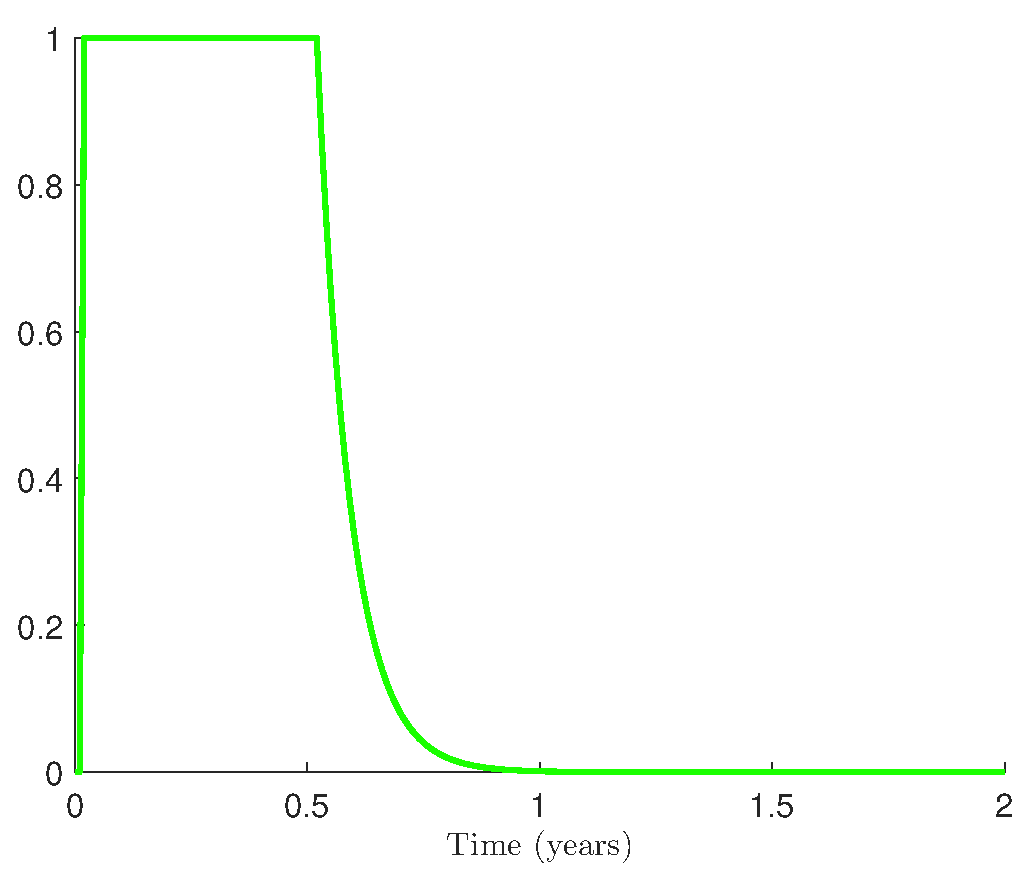
\includegraphics[width=0.75\textwidth]{DrugConc_19_04a.eps}
\caption{}
\label{drug} 
\end{figure*}


begin{figure*}
\begin{subfigure}{.5\textwidth}
  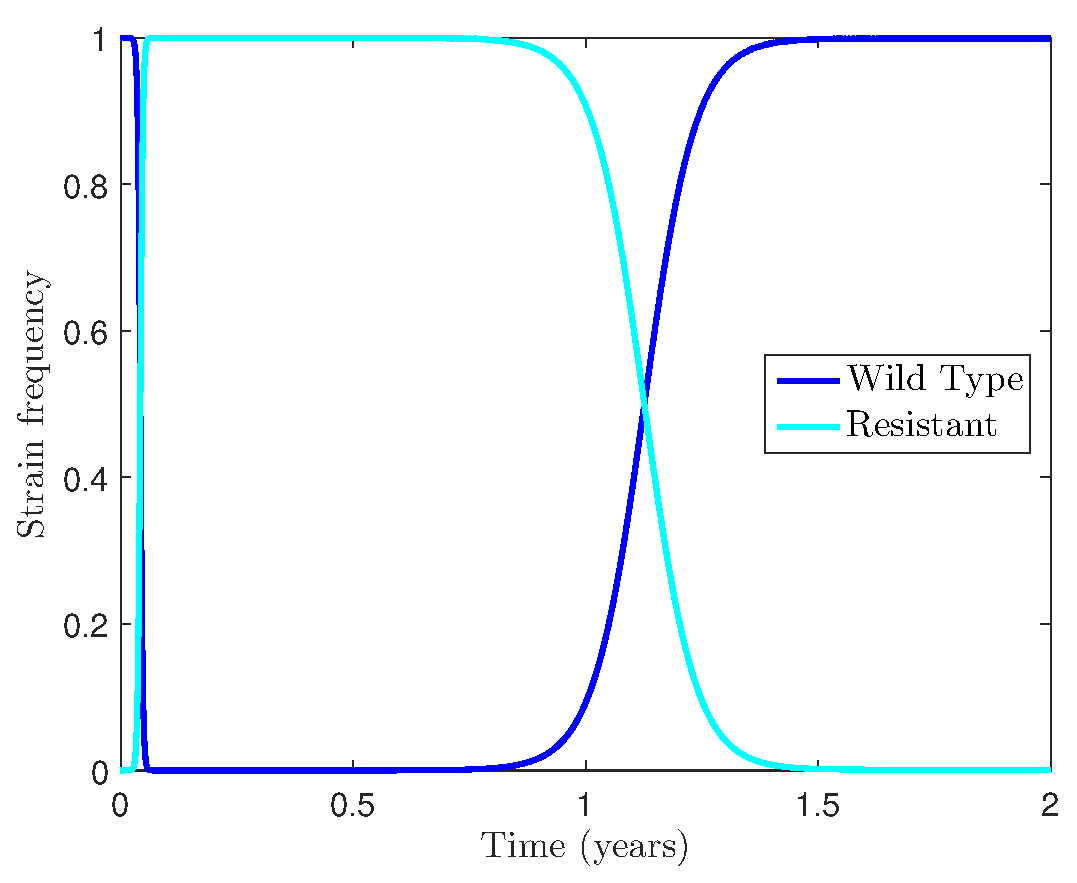
\includegraphics[width=.4\linewidth]{WithinHost_19_04a.eps}
\end{subfigure}%
\begin{subfigure}{.5\textwidth}
  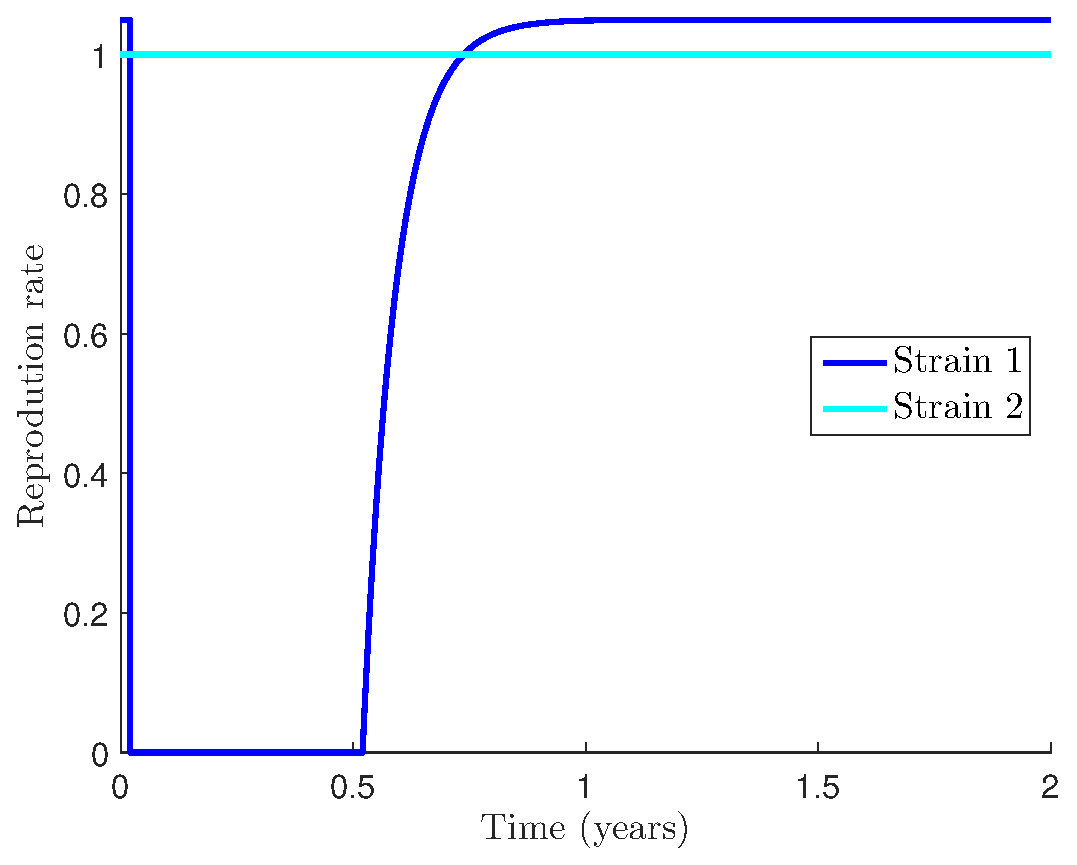
\includegraphics[width=.4\linewidth]{WithinHost_19_04b.eps}
\end{subfigure}
\caption{}
\label{fig:80}
\end{figure*}

Look at the effects of varying the reservoir parameters to see if the frequency in the active reservoir of the resistant strain can be increased. It can.

\iffalse
\begin{figure*}
  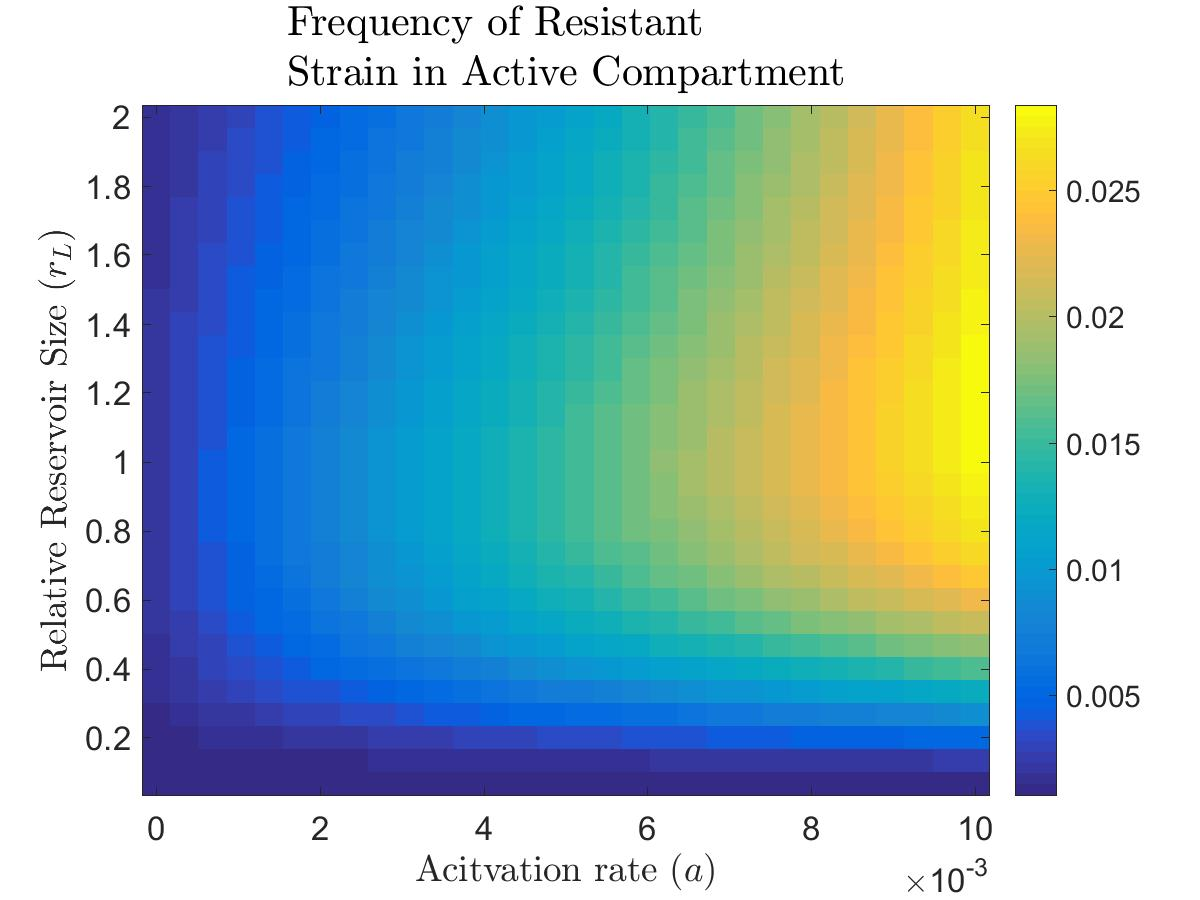
\includegraphics[width=0.75\textwidth]{FrequencyofResistantStraininActiveCompartment_19_04a.jpg}
\caption{Frequency of  the resistant strain present in the ctive compartment }
\label{fig:1} 
\end{figure*}
\fi

begin{figure*}
\begin{subfigure}{.5\textwidth}
  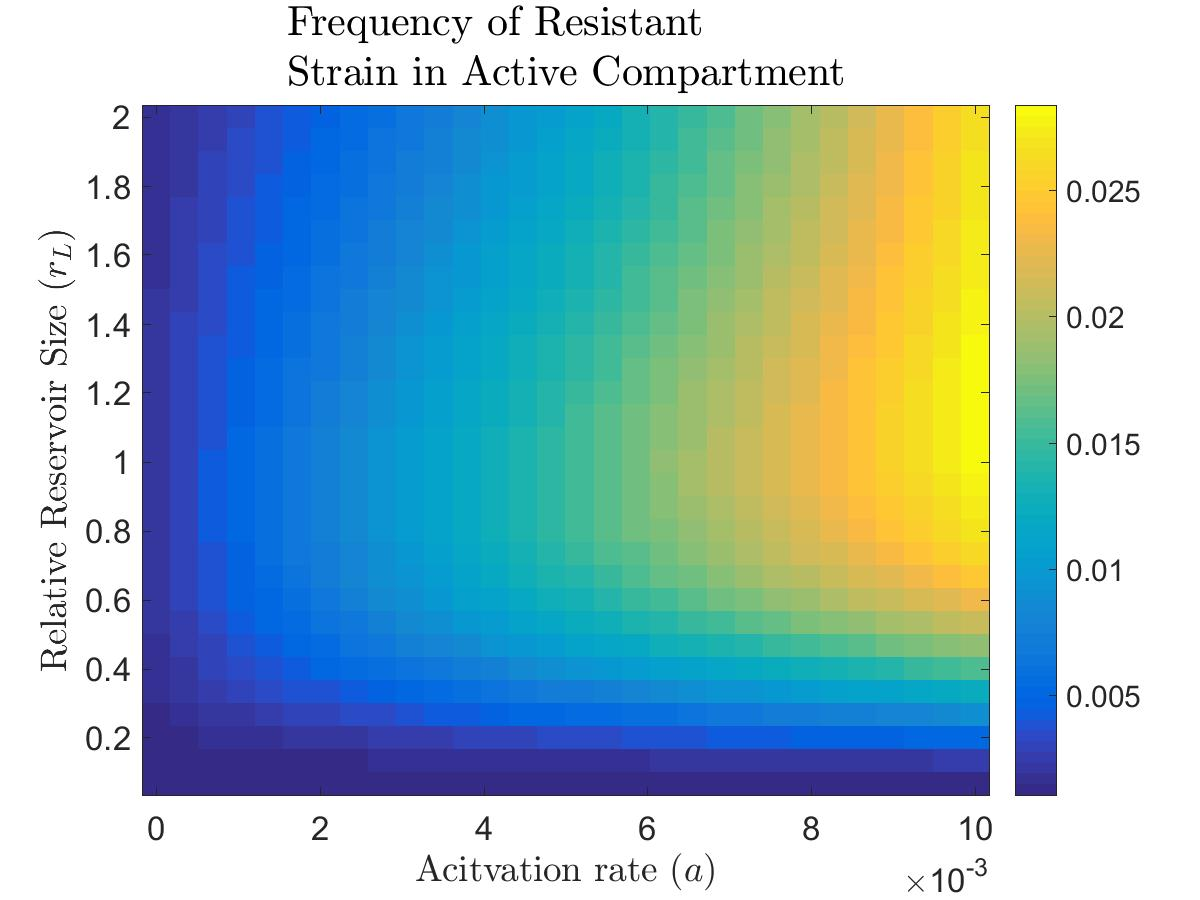
\includegraphics[width=.4\linewidth]{FrequencyofResistantStraininActiveCompartment_19_04a.jpg}
\end{subfigure}%
\begin{subfigure}{.5\textwidth}
  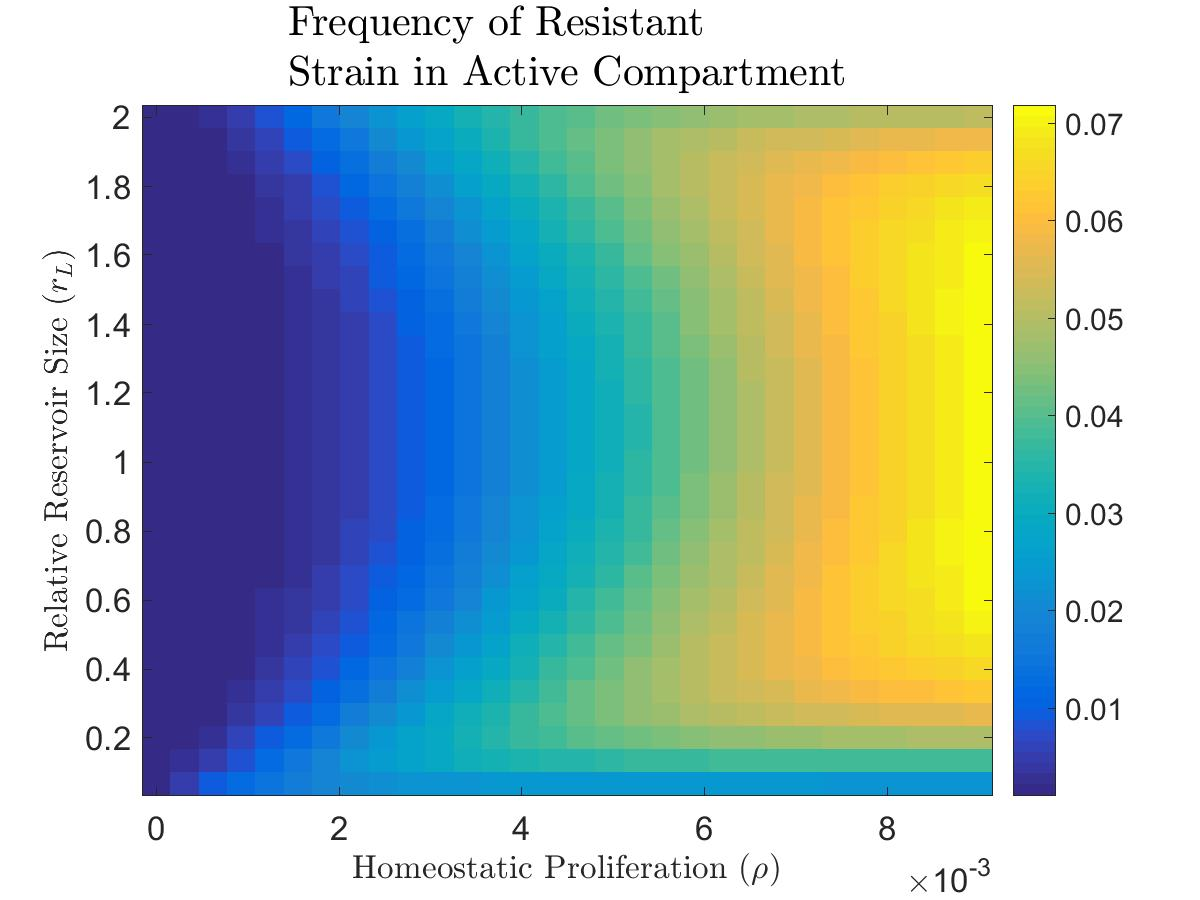
\includegraphics[width=.4\linewidth]{FrequencyofResistantStraininActiveCompartment_19_04b.jpg}
\end{subfigure}
\caption{Frequency of  the resistant strain present in the active compartment}
\label{fig:1}
\end{figure*}

\iffalse
\begin{figure*}
% Use the relevant command to insert your figure file.
% For example, with the graphicx package use
  \includegraphics[width=0.75\textwidth]{WithinMultiHost.eps}
% figure caption is below the figure
\caption{within host dynamics for two host two strain system. Top  two are in host not on the drug, where blue is the wild type and red is  the resistant strain. In the bottom two the host is on PrEP,as we are dealing with frequencies initiating wth the wild type  in a host on pRep GIVES A FREQUENCY  of 1 for  the wild type  (but this is just relative) soitmay be good either to set the frequency to 0 if the actual amount is small enough (so it not add to 1) or the infectivity will need to take account of both the host transmitting the virus and the host getting it.}
\label{fig:noh}       % Give a unique label
\end{figure*}
\fi


\bibliographystyle{apa}
\bibliography{DTCProject1Bibliography}   % name your BibTeX data base



 
\end{document}